

%\documentclass[a4paper]{jarticle}


\section{mgv.rb Create graph data for Graphviz (DOT) \label{sect:mgv}}
\index{mgv@mgv}

The graph data in CSV format is converted to a .dot file format for processing by Graphviz. 
 
Graph processing commands (e.g. mpolishing) contained in Take package reads and generates graphs expressed in CSV format. 
Visualization (graphic image) helps users to understand attributes of the graph, such as the scale and density. 
By converting graph data into DOT plain text graph description language, the graphs can be visualized in softwares such as Graphviz (\url{http://www.graphviz.org}) and Gephi (\url{http://www.gephi.org}). 

Graphviz is intended for the visualization of small graphs, thus, it may not be practical for large graphs with several hundred and thousands of vertices. 
It is recommended  to use Gephi for drawing of large-scale  graphs. 

 

\subsection{Format}
\begin{verbatim}
mgv.rb [ni=] [nf=] [nv=] [nr=] [-nl] ei= ef= [ev=] [er=] [-el] [-d] [o=] [--help]
\end{verbatim}

\begin{table}[htbp]
{\small
\begin{tabular}{ll}
\verb|ni=| & : File name of vertex set \\
\verb|nf=| & : Field name of vertex  \\
\verb|nv=| & : Field name of vertex attribute (size of vertex)   \\
\verb|nr=| & : Enlargement ratio when drawing graph. This parameter accepts integer values from 1 to 10. Default is set at 3 \\
\verb|-nl| & : Specified value at \verb|nv=| is added to the node name  \\
\verb|ei=| & : File name of edge set  \\
\verb|ef=| & : ID field name of beginning vertex and end vertex  \\
\verb|ev=| & : Field name of edge attribute (thickness of edge)  \\
\verb|er=| & : Enlargement ratio of edge when drawing graph. This parameter accepts integer values from 1 to 10. Default is set at 10.  \\
\verb|-el| & : Show width of edge specified at  \verb|ev=|  \\
\verb|-d|  & : Specify directed graph   \\
\verb|o=|  & : Output file name (.dot file)   \\
\verb|--help| & : Show help  \\
\end{tabular} 
}
\end{table} 


The input graph data may only be specified  at \verb|ei=| parameter as edge set CSV data.  
In order to include the attribute of vertices (size), the CSV data of the vertices set used can be specified at \verb|ni=| parameter.  


\subsubsection*{Display graph data in CSV format }

One row represents one edge, which corresponds to the start of vertex and end of vertex stored in two fields. 


\begin{Verbatim}[baselinestretch=0.7,frame=single]
node1,node2
A,B
B,C
C,A
C,D
E,D
\end{Verbatim}

\subsubsection*{Example of .dot format graph data}

Contains information related to vertices and information of edges. 

\begin{Verbatim}[baselinestretch=0.7,frame=single]
digraph G { 
  edge [dir=none]

    n0 [label="A" height=0.5 width=0.75] 
n1 [label="B" height=0.5 width=0.75] 
n2 [label="C" height=0.5 width=0.75] 
n3 [label="D" height=0.5 width=0.75] 
n4 [label="E" height=0.5 width=0.75] 


    n0 -> n1 [style="setlinewidth(1.0)"]
n1 -> n2 [style="setlinewidth(1.0)"]
n2 -> n0 [style="setlinewidth(1.0)"]
n2 -> n3 [style="setlinewidth(1.0)"]
n4 -> n3 [style="setlinewidth(1.0)"]

}
\end{Verbatim}

\subsubsection*{Example to draw by Graphviz}

Graphviz GUI allows users to interact with graph data, the \verb|dot| command installed with Graphviz allows for conversion to graphic (.png file). The visual of graph is shown in diagram \ref{fig:mgv0}. 


\begin{Verbatim}[baselinestretch=0.7,frame=single]
$ dot -Tpng rsl1.dot > rsl1.png
$ open rsl1.png
\end{Verbatim}

\begin{figure}[htbp]
\begin{center}
\begin{tabular}{c}

\begin{minipage}{1.0\hsize}
\begin{center}
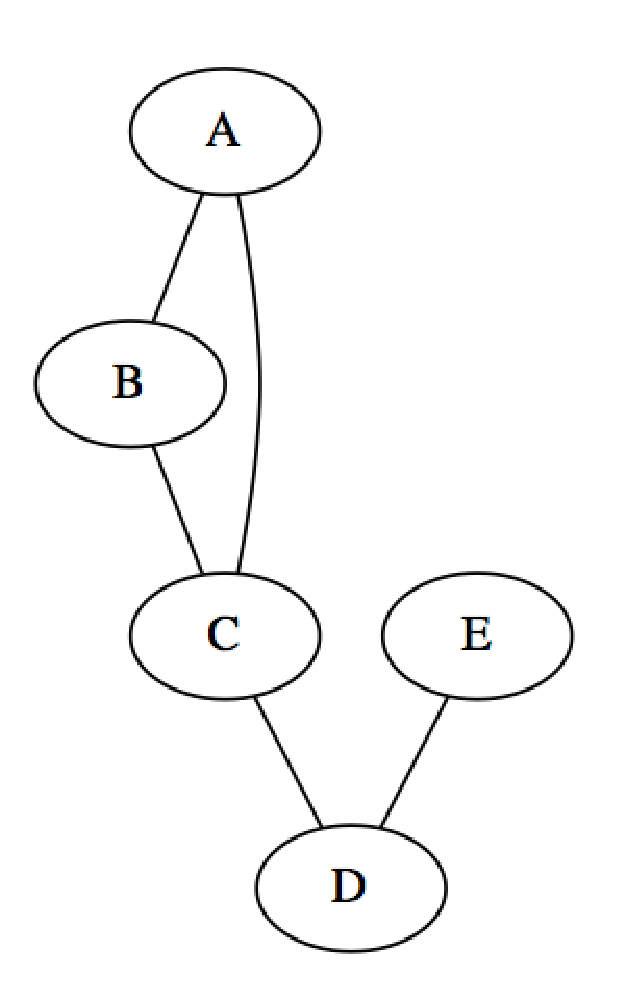
\includegraphics[scale=0.5]{figure/mgv0.eps}
\caption{Example of drawing with Graphviz \label{fig:mgv0}}
\end{center}
\end{minipage}

\end{tabular}
\end{center}
\end{figure}

\newpage
\subsection{Examples}
\subsubsection*{例1: 基本例}

開始頂点と終了頂点からなる枝集合ファイルのみを与える。


\begin{Verbatim}[baselinestretch=0.7,frame=single]
$ more edge1.csv
node1,node2
A,B
B,C
C,A
C,D
E,D
$ mgv.rb ei=edge1.csv ef=node1,node2 o=rsl1.dot
\end{Verbatim}
\begin{minipage}{1.0\hsize}
\begin{center}
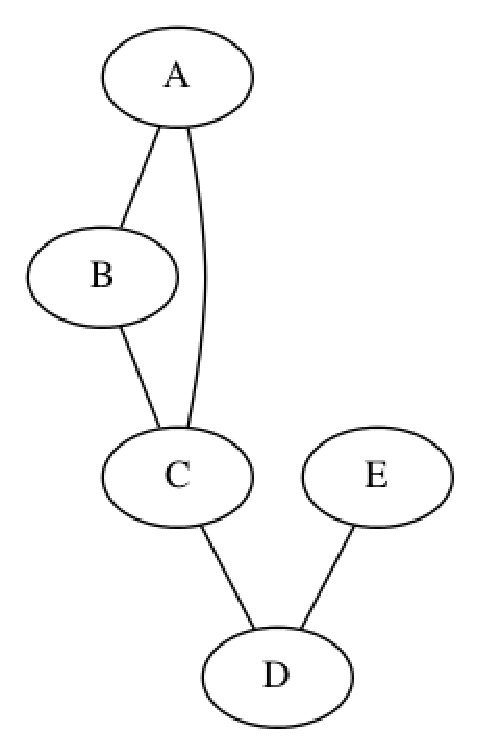
\includegraphics[scale=0.5]{figure/mgv1.eps}
\end{center}
\end{minipage}
\subsubsection*{例2: 枝に属性(太さ)を指定する例}

\verb|ev=|パラメータで\verb|val|項目を属性(太さ)として指定している。
同時に\verb|-el|オプションを付けることで、属性値もグラフに描画される。


\begin{Verbatim}[baselinestretch=0.7,frame=single]
$ more edge2.csv
node1,node2,val
A,B,10
B,C,20
C,A,30
C,D,40
E,D,20
$ mgv.rb ei=edge2.csv ef=node1,node2 ev=val -el o=rsl2.dot
\end{Verbatim}
\begin{minipage}{1.0\hsize}
\begin{center}
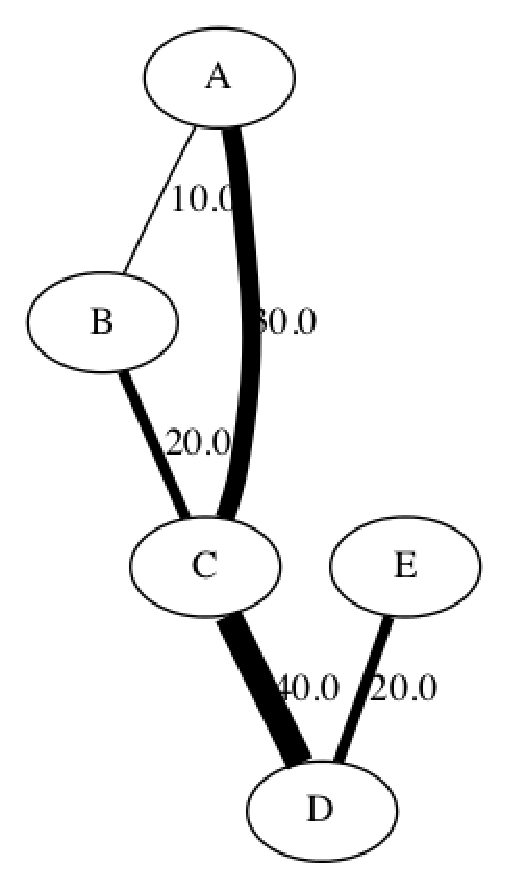
\includegraphics[scale=0.5]{figure/mgv2.eps}
\end{center}
\end{minipage}
\subsubsection*{例3: 頂点に属性(大きさ)を指定する例}

\verb|ni=|パラメータで頂点集合ファイルを指定する。
\verb|nv=|パラメータで、\verb|val|項目を属性(大きさ)として指定している。


\begin{Verbatim}[baselinestretch=0.7,frame=single]
$ more node1.csv
node,val
A,10
B,15
C,8
D,5
E,20
$ more edge1.csv
node1,node2
A,B
B,C
C,A
C,D
E,D
$ mgv.rb ei=edge1.csv ef=node1,node2 ni=node1.csv nf=node nv=val o=rsl3.dot
\end{Verbatim}
\begin{minipage}{1.0\hsize}
\begin{center}
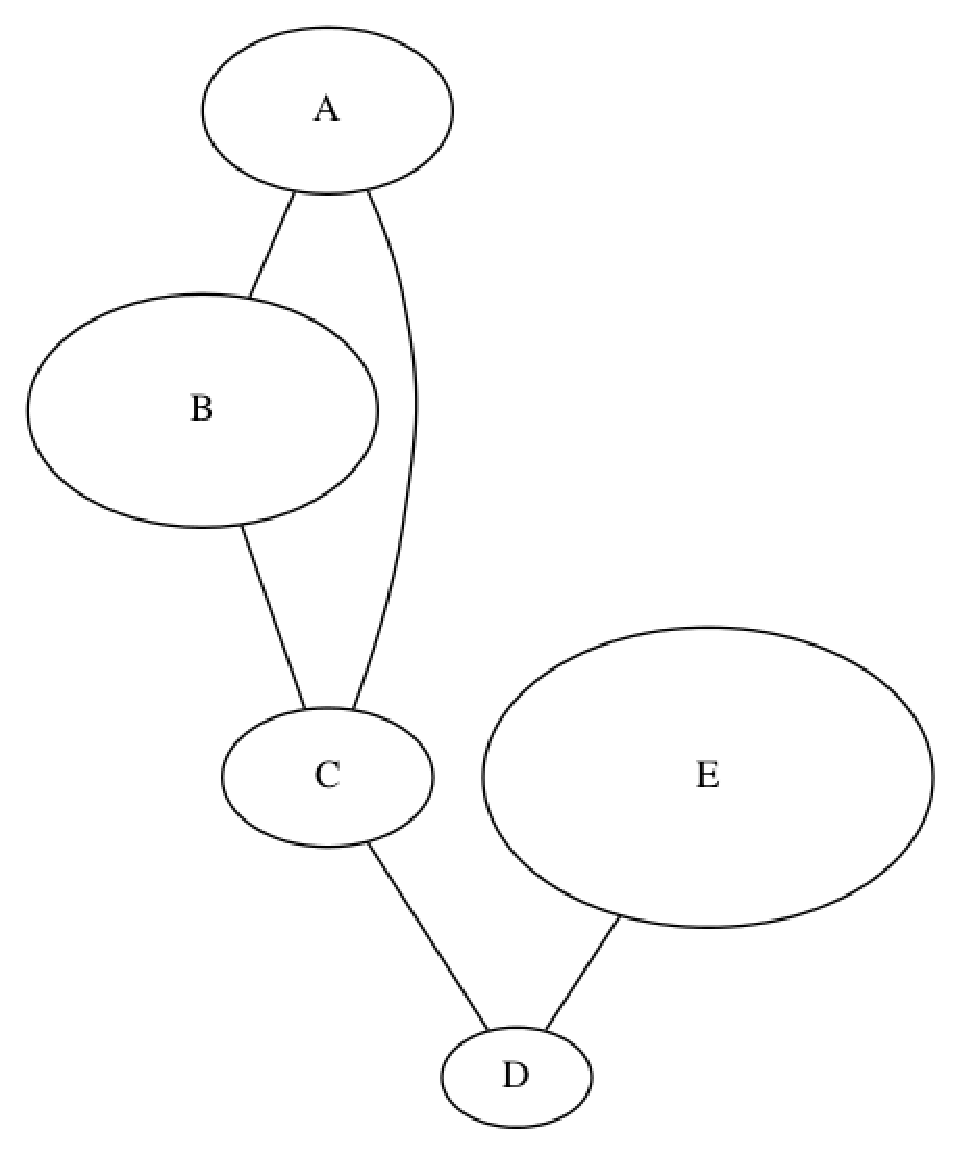
\includegraphics[scale=0.3]{figure/mgv3.eps}
\end{center}
\end{minipage}
\subsubsection*{例4: 頂点に属性(大きさ)と拡大率を指定する例}

\verb|nr=|パラメータで、ノードの拡大率を指定している。


\begin{Verbatim}[baselinestretch=0.7,frame=single]
$ more node1.csv
node,val
A,10
B,15
C,8
D,5
E,20
$ more edge1.csv
node1,node2
A,B
B,C
C,A
C,D
E,D
$ mgv.rb ei=edge1.csv ef=node1,node2 ni=node1.csv nf=node nv=val nr=5 o=rsl4.dot
\end{Verbatim}
\begin{minipage}{1.0\hsize}
\begin{center}
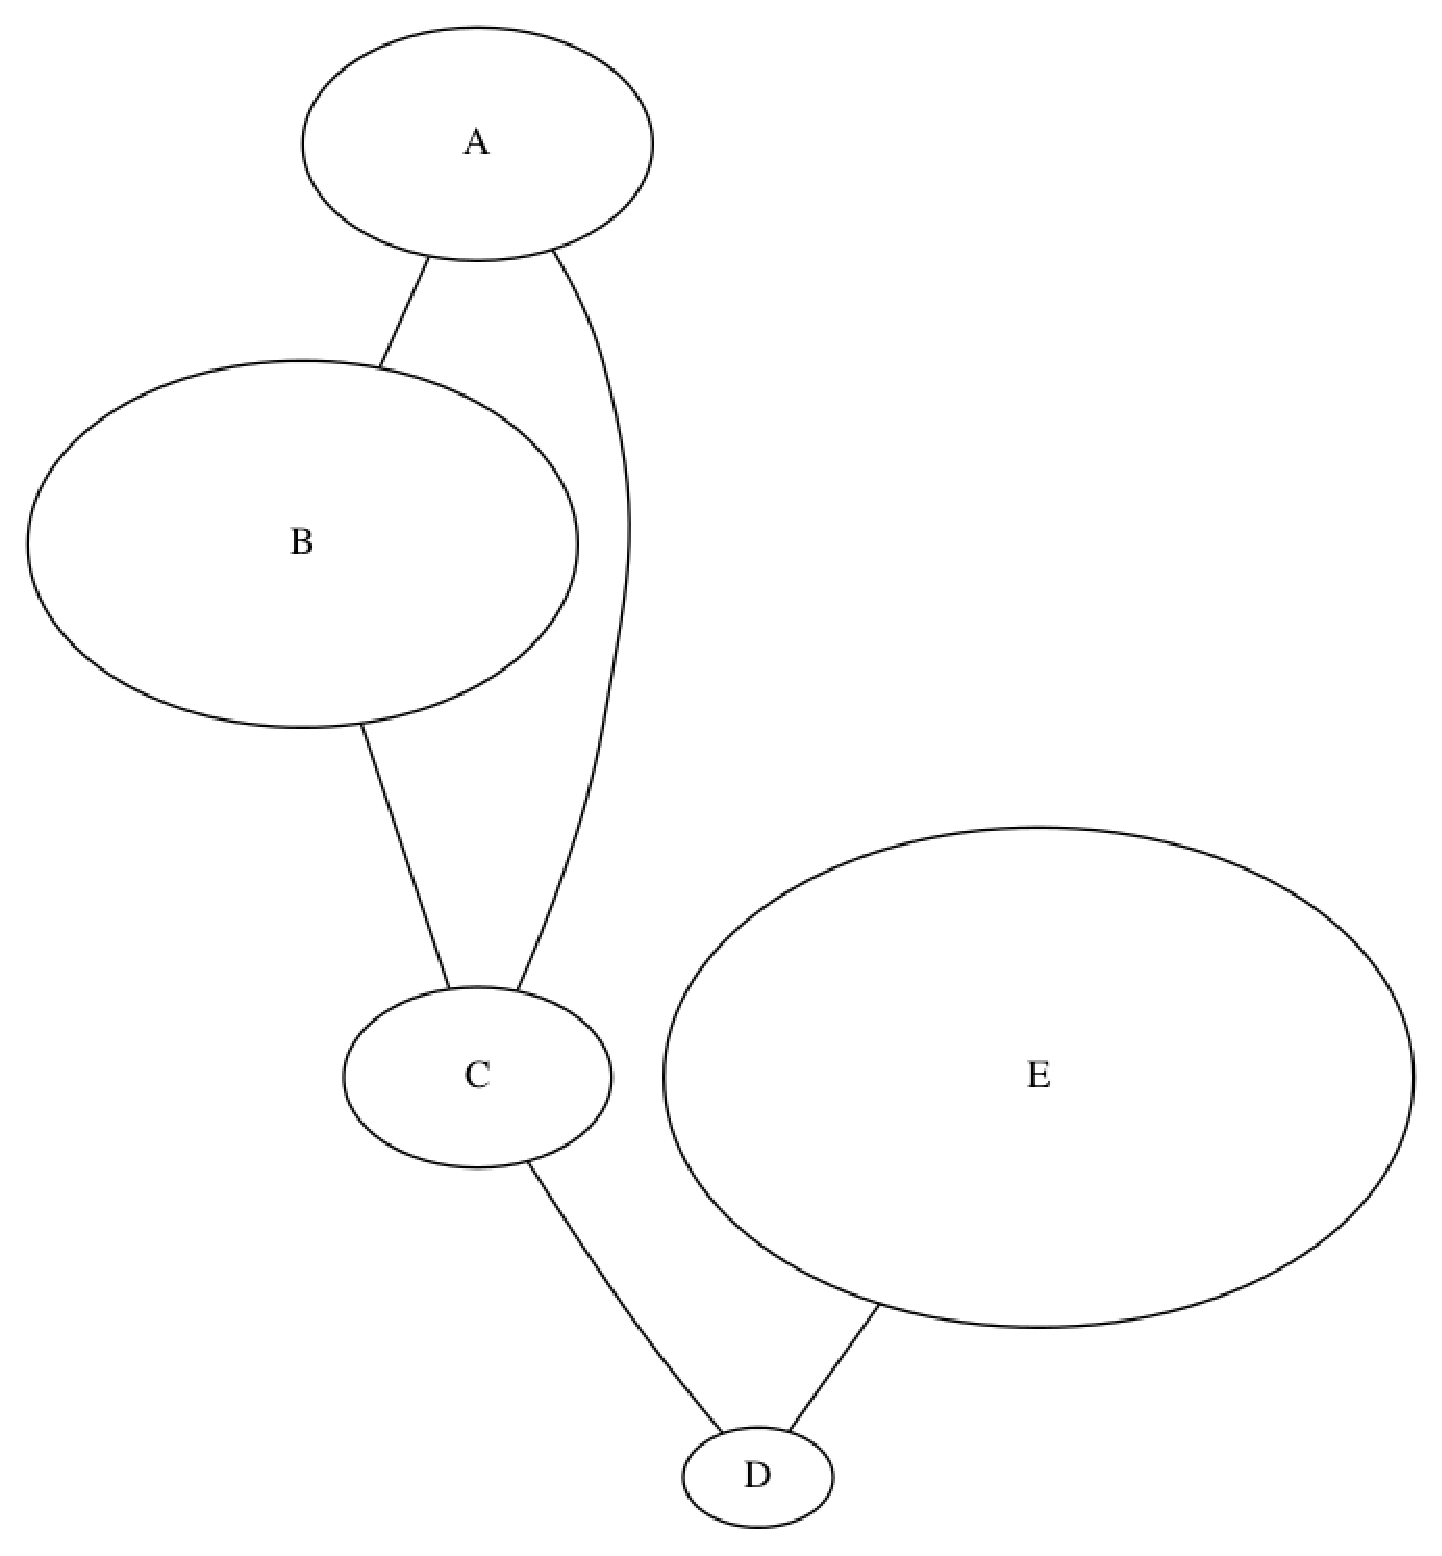
\includegraphics[scale=0.3]{figure/mgv4.eps}
\end{center}
\end{minipage}


%\end{document}

